\documentclass[11pt,a4paper]{article}
\usepackage{fontspec}
\setmainfont{Times New Roman}
\usepackage[spanish,es-tabla]{babel}
\usepackage[margin=2.3cm,headheight=15pt]{geometry}
\usepackage{booktabs,tabularx,array,graphicx}
\usepackage{enumitem,setspace,fancyhdr,titlesec}
\usepackage[hidelinks,unicode]{hyperref}
\setstretch{1.12}
\setlength{\parindent}{0pt}
\setlength{\parskip}{6pt}
\setlist[itemize]{leftmargin=*,nosep,topsep=4pt}
\setlist[enumerate]{leftmargin=*,itemsep=3pt,topsep=4pt}
\renewcommand{\arraystretch}{1.22}
\newcolumntype{Y}{>{\raggedright\arraybackslash}X}
\newcolumntype{P}[1]{>{\raggedright\arraybackslash}p{#1}}
\titleformat{\section}{\Large\bfseries}{\thesection.}{.6em}{}
\titleformat{\subsection}{\normalsize\bfseries}{\thesubsection}{.6em}{}
\titlespacing*{\section}{0pt}{0pt}{14pt}
\titlespacing*{\subsection}{0pt}{12pt}{5pt}
\pagestyle{fancy}
\fancyhf{}
\fancyhead[L]{\small DS3031 / Laboratorio 11}
\fancyhead[R]{\small Registro de personas}
\fancyfoot[L]{\footnotesize Ronal Condor Blas}
\fancyfoot[R]{\footnotesize\thepage}
\renewcommand{\headrulewidth}{.3pt}
\hypersetup{pdftitle={Laboratorio 11: Registro de personas y evaluación de impacto en privacidad},pdfauthor={Ronal Condor Blas}}
\emergencystretch=2em
\newcommand{\repo}{https://github.com/ronaljcb/lab11-registro-privacidad}
\newcommand{\sitio}{https://lab11-registro-privacidad.vercel.app}
\begin{document}
\thispagestyle{empty}
{\small DS3031\hfill ÉTICA Y SEGURIDAD DE LOS DATOS}

\vspace{1.2cm}\hrule\vspace{1cm}
{\large LABORATORIO 11 / HANDS-ON}

\vspace{.6cm}
{\Huge\bfseries Registro de personas}

\vspace{.35cm}
{\LARGE Evaluación de impacto en privacidad}

\vspace{.8cm}
{\large Informe técnico y DPIA}

\vspace{1.1cm}
\begin{tabular}{@{}ll}
\textbf{Responsable} & Ronal Condor Blas\\[5pt]
\textbf{Modalidad de elaboración} & Individual\\[5pt]
\textbf{Fecha} & 24 de octubre de 2026\\[5pt]
\textbf{Alcance} & Demostración académica con datos ficticios\\
\end{tabular}

\vspace{1cm}
\textbf{Resumen}

Se implementó un registro de personas con frontend en Next.js y componentes shadcn/ui, una API del servidor y una base PostgreSQL en Neon. El sistema registra nombres, apellidos, correo y teléfono; este último campo es opcional. La aplicación permite consultar y eliminar los registros de la propia sesión.

La evaluación analiza los riesgos del backend mínimo y los relaciona con restricciones verificables. La demostración incluye aislamiento por sesión, validación del servidor, consultas parametrizadas y control de solicitudes. Estas medidas no sustituyen una autenticación de usuarios ni acreditan cumplimiento normativo para un servicio con datos reales.

\textbf{Decisión:} habilitar la demostración únicamente con datos ficticios. El tratamiento de datos reales requiere resolver las condiciones pendientes de la sección 5.

\vfill
\textbf{Accesos a la entrega}

Aplicación: \url{\sitio}

Código y documentación: \url{\repo}

\vspace{.5cm}\hrule
{\footnotesize La revisión cruzada de otro grupo está pendiente. La modalidad individual debe ser aceptada por el docente; este informe no presupone dicha autorización.}

\newpage
\section{Descripción del tratamiento}
\subsection{Finalidad y límites}
El sistema reproduce el flujo de alta, consulta y eliminación de un directorio pequeño para analizar decisiones de privacidad. No envía correos, mensajes ni llamadas. No administra matrículas, asistencia o información real de alumnos. Los ejemplos corresponden a identidades inventadas.

El backend exige correos terminados en \texttt{@example.com}. El teléfono, si se ingresa, debe tener nueve dígitos y empezar con \texttt{000}. La confirmación del formulario declara el uso de datos ficticios; no constituye consentimiento para tratar información personal real.

\subsection{Componentes y flujo}
\begin{enumerate}
\item El navegador muestra el formulario y envía una solicitud JSON al mismo origen.
\item La API valida los campos, el origen de la solicitud y la sesión vigente.
\item El servidor consulta PostgreSQL mediante la credencial de Neon, guardada como variable de entorno.
\item La respuesta devuelve únicamente los registros asociados con la sesión del navegador. El listado no utiliza caché compartida.
\end{enumerate}
Vercel aloja el frontend y las funciones del servidor. Neon aloja PostgreSQL en la región configurada \texttt{iad1}, Estados Unidos. GitHub conserva el código y la documentación, sin la base de datos ni las credenciales.

\subsection{Inventario de datos}
{\small
\renewcommand{\arraystretch}{1.08}
\begin{tabularx}{\textwidth}{@{}P{2.2cm}YP{2.5cm}P{2.9cm}@{}}
\toprule
\textbf{Campo} & \textbf{Uso y clasificación en un sistema real} & \textbf{Necesidad} & \textbf{Acceso / conservación}\\
\midrule
Nombres y apellidos & Identificación de la persona; datos identificativos. & Requeridos para distinguir registros. & Solo la sesión; acceso hasta su vencimiento.\\
Correo & Identificador de contacto; dato personal. En la demo usa dominio reservado. & Requerido para formato y unicidad por sesión. & Solo la sesión; sin envíos de correo.\\
Teléfono & Contacto adicional; dato personal. En la demo usa numeración inválida. & Opcional; no se necesita para completar el flujo. & Solo la sesión; puede ser nulo.\\
Identificador UUID & Localiza el registro sin un consecutivo público. & Necesidad técnica. & API y base; vinculado a la sesión.\\
Huella de sesión & SHA-256 de un token aleatorio de 256 bits. Es pseudónima, no anónima. & Delimitar lectura y eliminación. & Solo servidor y base.\\
Fechas y contadores & Creación, vencimiento y límite de solicitudes. & Caducidad y control operativo. & Solo servidor; sin listados públicos.\\
\bottomrule
\end{tabularx}}
No se solicitan DNI, ubicación, edad, archivos ni categorías sensibles. Los proveedores pueden procesar metadatos técnicos de conexión de acuerdo con sus políticas.

\newpage
\section{Necesidad y proporcionalidad}
\subsection{Decisiones por campo}
\begin{tabularx}{\textwidth}{@{}P{2.4cm}YY@{}}
\toprule
\textbf{Dato} & \textbf{Justificación en la práctica} & \textbf{Decisión de minimización}\\
\midrule
Nombres y apellidos & Permiten comprobar el registro de una persona y la visualización de texto. & Máximo 60 caracteres por campo. No se pide documento de identidad.\\
Correo & Permite validar formato y detectar duplicados dentro de una sesión. & Solo \texttt{@example.com}; no se verifica identidad ni se contacta al titular.\\
Teléfono & Se incluye por la consigna y permite estudiar un dato adicional de contacto. & Opcional. Se almacena \texttt{NULL} cuando se omite.\\
Sesión y fechas & Permiten delimitar el acceso y evaluar retención. & Cookie necesaria, sin analítica publicitaria ni rastreo entre sitios.\\
\bottomrule
\end{tabularx}

\subsection{Ciclo de vida del dato}
\textbf{Recolección.} Formulario visible con finalidad y advertencia de datos ficticios. La validación ocurre también en el servidor; cambiar el HTML no permite omitirla.

\textbf{Almacenamiento y uso.} Los datos se guardan en PostgreSQL y se utilizan para mostrar el listado de la sesión. La credencial de la base permanece en el servidor. El token bruto de sesión queda en la cookie; la tabla conserva su huella.

\textbf{Comunicación.} El navegador se comunica con el origen de la aplicación. La función del servidor accede a Neon. No hay exportación pública ni endpoint que liste todas las sesiones.

\textbf{Retención.} La sesión y los registros tienen un vencimiento a las 24 horas. Las consultas excluyen los datos vencidos. La caducidad de acceso no equivale a eliminación física: se proporciona el comando \texttt{npm run db:cleanup} para eliminar sesiones vencidas y sus registros en cascada. Su programación periódica sigue pendiente.

\textbf{Eliminación.} El usuario puede borrar un registro de su sesión. La API comprueba la propiedad en la misma consulta SQL. Las copias de respaldo y su retención dependen del proveedor y requieren una política específica antes del uso real.

\subsection{Marco de evaluación}
Se utiliza la estructura académica del laboratorio: descripción, necesidad, riesgos, medidas, riesgo residual y decisión. La Ley N.\textsuperscript{o} 29733 y su reglamento, así como el GDPR tratado en clase, orientan las preguntas de diseño. Este documento no certifica cumplimiento legal ni asume que publicar un aviso o marcar una casilla sea suficiente.

Una aplicación real necesitaría identificar al responsable del tratamiento, precisar la finalidad y su base jurídica, definir los destinatarios y transferencias, habilitar la atención de derechos y revisar los acuerdos con los proveedores. Estas cuestiones se mantienen como condiciones de lanzamiento.

\newpage
\section{Riesgos del backend mínimo}
Los riesgos iniciales corresponden al escenario previo a los controles, considerando el posible uso de nombres y datos de contacto reales. No son afirmaciones de vulnerabilidades actualmente reproducidas.

\textbf{Escala.} Probabilidad (P) e impacto (I): 1 bajo, 2 medio y 3 alto. Puntaje $P\times I$: 1--3 bajo, 4--6 medio y 7--9 alto. La valoración es cualitativa y no expresa una probabilidad estadística.

{\small
\begin{tabularx}{\textwidth}{@{}P{.7cm}YP{2.1cm}ccc@{}}
\toprule
\textbf{ID} & \textbf{Escenario concreto y consecuencia} & \textbf{LINDDUN} & \textbf{P} & \textbf{I} & \textbf{Nivel}\\
\midrule
R1 & Un visitante consulta el listado de otra sesión y obtiene nombres, correos y teléfonos. & Disclosure & 3 & 3 & 9 Alto\\
R2 & Una persona reutiliza el mismo navegador o copia su cookie y accede a los registros ajenos. & Disclosure, linkability & 2 & 3 & 6 Medio\\
R3 & El formulario obliga a entregar un teléfono sin una finalidad adicional necesaria. & Unawareness, non-compliance & 2 & 2 & 4 Medio\\
R4 & Una entrada se concatena en una consulta SQL y permite leer o alterar registros. & Disclosure & 3 & 3 & 9 Alto\\
R5 & Una credencial o un volcado de datos se publica en GitHub y habilita acceso a la base. & Disclosure & 2 & 3 & 6 Medio\\
R6 & Los registros permanecen indefinidamente porque se confunde vencimiento de sesión con borrado. & Non-compliance & 3 & 2 & 6 Medio\\
R7 & El sistema usa proveedores en otro país sin analizar destinatarios, transferencias y condiciones. & Non-compliance & 2 & 3 & 6 Medio\\
R8 & Los logs incluyen el JSON del formulario, cookies o parámetros SQL y amplían la exposición. & Disclosure & 2 & 2 & 4 Medio\\
R9 & Un sitio externo provoca altas o eliminaciones utilizando la sesión del navegador. & Non-compliance & 2 & 3 & 6 Medio\\
R10 & Un atacante crea muchas sesiones y consume la cuota del servicio, afectando su disponibilidad. & Non-compliance & 3 & 2 & 6 Medio\\
\bottomrule
\end{tabularx}}

\subsection{Criterio de priorización}
R1 y R4 requieren restricciones antes de exponer una API en Internet. Los riesgos medios también reciben medidas verificables. Los registros de cada sesión no deben aparecer en respuestas ajenas, y una entrada válida nunca debe convertirse en código SQL.

La pseudonimización de la sesión disminuye la exposición del token en la base, pero no anonimiza los registros. El control por cookie tampoco verifica la identidad de una persona.

\newpage
\section{Restricciones de diseño verificables}
{\small
\begin{tabularx}{\textwidth}{@{}P{.7cm}P{.9cm}YP{2.1cm}@{}}
\toprule
\textbf{ID} & \textbf{R.} & \textbf{Restricción y forma de comprobarla} & \textbf{Estado}\\
\midrule
C1 & R1 & Toda lectura y eliminación debe filtrar por la huella de la sesión vigente. Una sesión B no lista ni elimina un UUID creado por A; recibe 404 al intentar borrarlo. & Implementada y probada.\\
C2 & R2 & Token aleatorio de 32 bytes; cookie HttpOnly, SameSite=Strict y Secure en producción; vigencia de 24 horas. Comprobar cabecera Set-Cookie y rechazo de sesión vencida. & Implementada; autenticación personal pendiente.\\
C3 & R3 & El teléfono debe ser opcional en UI, API y base. Un alta con cadena vacía debe guardar NULL y devolver 201. & Implementada y probada.\\
C4 & R4 & Consultas SQL parametrizadas; validación estricta de campos y tipos en el servidor. No concatenar entradas a sentencias SQL. & Implementada y revisada.\\
C5 & R5 & Credenciales solo en variables del servidor. Excluir .env, .vercel, .db y .sqlite. Verificar archivos seguidos antes del push. & Implementada; rotación periódica pendiente.\\
C6 & R6 & Excluir datos vencidos de toda consulta y ofrecer limpieza en cascada. Antes del uso real, programar el borrado y definir retención de respaldos. & Acceso limitado; limpieza manual disponible.\\
C7 & R7 & Documentar proveedor y región. Antes del uso real, revisar contratos, destinatarios, transferencias y base jurídica con el responsable. & Documentada; revisión jurídica pendiente.\\
C8 & R8 & No registrar payloads, cookies, credenciales ni parámetros SQL. Los errores guardan solo un código técnico y el cliente recibe un mensaje genérico. & Implementada; política del proveedor pendiente.\\
C9 & R9 & POST y DELETE requieren origen idéntico y sesión. POST exige JSON y limita el cuerpo a 2 KB. Un origen externo debe devolver 403. & Implementada y probada.\\
C10 & R10 & Máximo 20 mutaciones por minuto y 50 registros por sesión, controlados en la base. Antes del uso real, agregar protección global contra creación masiva de sesiones. & Límite por sesión implementado; global pendiente.\\
\bottomrule
\end{tabularx}}

\subsection{Alcance de implementación}
La consigna permite escribir las restricciones sin implementarlas. En esta entrega se implementó un subconjunto para desplegar una demostración funcional. La columna de estado diferencia lo comprobado de las condiciones todavía pendientes.

No se promete borrado automático de la base ni autenticación de personas. El aviso de privacidad de la aplicación explica ambas limitaciones.

\newpage
\section{Riesgo residual y decisión}
La siguiente matriz evalúa el sistema con los controles implementados y conserva el impacto de un escenario con datos reales. Las condiciones no implementadas no se consideran resueltas.

{\small
\begin{tabularx}{\textwidth}{@{}P{1cm}P{1.5cm}P{1.2cm}P{1.2cm}P{1.8cm}Y@{}}
\toprule
\textbf{Riesgo} & \textbf{Control} & \textbf{P final} & \textbf{I final} & \textbf{Residual} & \textbf{Justificación}\\
\midrule
R1 & C1 & 1 & 3 & 3 Bajo & Filtro del servidor y prueba entre dos sesiones.\\
R2 & C2 & 2 & 3 & 6 Medio & Cookie protegida; compartir navegador sigue dando acceso.\\
R3 & C3 & 1 & 2 & 2 Bajo & El teléfono puede omitirse sin impedir el alta.\\
R4 & C4 & 1 & 3 & 3 Bajo & Validación y consultas con parámetros.\\
R5 & C5 & 1 & 3 & 3 Bajo & Sin secretos ni base de datos en el repositorio.\\
R6 & C6 & 2 & 2 & 4 Medio & Caducidad de acceso; borrado programado pendiente.\\
R7 & C7 & 2 & 3 & 6 Medio & Proveedores identificados; análisis jurídico pendiente.\\
R8 & C8 & 1 & 2 & 2 Bajo & Logs de aplicación mínimos; metadatos del proveedor.\\
R9 & C9 & 1 & 3 & 3 Bajo & Origen, sesión y formato comprobados.\\
R10 & C10 & 2 & 2 & 4 Medio & Cuota por sesión; se pueden generar sesiones nuevas.\\
\bottomrule
\end{tabularx}}

\subsection{Decisión de lanzamiento}
\textbf{Se puede publicar la demostración con condiciones: exclusivamente datos ficticios, finalidad académica y advertencia visible. No se autoriza el uso de datos personales reales.}

El servidor exige formatos ficticios para correo y teléfono. La aplicación no puede demostrar que un nombre escrito sea inventado, por lo que la advertencia y la responsabilidad de quien prueba el sistema siguen siendo necesarias.

\subsection{Condiciones para un eventual uso real}
\begin{enumerate}
\item Sustituir la sesión anónima por autenticación y autorización adecuadas al servicio; definir roles y recuperación de acceso.
\item Precisar responsable, finalidad y base jurídica, información al titular, atención de derechos y condiciones con proveedores.
\item Programar y supervisar el borrado, establecer retención de respaldos y documentar el manejo de incidentes.
\item Añadir controles globales de abuso, límites por servicio y seguimiento de consumo.
\item Revaluar los riesgos con el flujo real y recibir una revisión independiente antes de ampliar el alcance.
\end{enumerate}
\textbf{Responsable de esta decisión académica:} Ronal Condor Blas.

\textbf{Fecha:} 24 de octubre de 2026. La identificación del responsable es una constancia en el informe; no se presenta como firma digital ni aprobación de otro grupo.

\newpage
\section{Verificación técnica y evidencia}
\subsection{Flujo comprobado}
La verificación recorre interfaz, API, persistencia y respuesta. El script \texttt{scripts/verify-api.mjs} ejecuta doce comprobaciones y puede repetirse contra el despliegue mediante la variable \texttt{BASE\_URL}.

{\small
\begin{tabularx}{\textwidth}{@{}P{.7cm}YP{3.2cm}@{}}
\toprule
\textbf{N.} & \textbf{Comprobación} & \textbf{Resultado esperado y verificado}\\
\midrule
1 & Cookie de sesión y ausencia de caché compartida. & Cookie emitida; no-store.\\
2 & Alta persistente de persona ficticia. & HTTP 201 y UUID.\\
3 & Lectura después del alta. & El registro aparece.\\
4 & Otra sesión no lista ni elimina el registro. & Lista aislada; DELETE 404.\\
5 & Correo duplicado en una sesión. & HTTP 409.\\
6 & Correo real, teléfono real o confirmación ausente. & HTTP 400.\\
7 & Mutación sin sesión o con origen externo. & HTTP 401 / 403.\\
8 & JSON inválido o cuerpo mayor que 2 KB. & HTTP 400 / 413.\\
9 & Alta sin teléfono. & HTTP 201; teléfono nulo.\\
10 & Eliminación y lectura posterior. & HTTP 200; registro ausente.\\
11 & Solicitud 21 dentro del minuto. & HTTP 429; Retry-After.\\
12 & Estado de la conexión con la base. & Health HTTP 200.\\
\bottomrule
\end{tabularx}}

\subsection{Interfaz del registro}
\IfFileExists{images/tabla-registro.jpg}{\begin{center}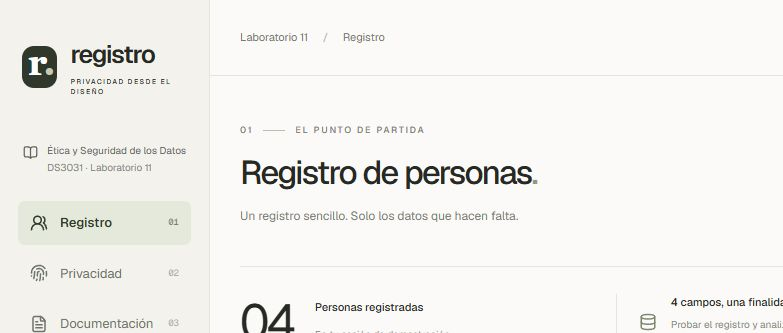
\includegraphics[width=\textwidth,height=6.1cm,keepaspectratio]{images/tabla-registro.jpg}\end{center}}{\textit{La captura de la interfaz se incorpora en la versión final del informe.}}
{\footnotesize Figura 1. Registro con ejemplos ficticios. La interfaz utiliza componentes shadcn/ui y mantiene el teléfono como campo opcional.}

\newpage
\section{Entrega, revisión y referencias}
\subsection{Checklist de la entrega}
{\small
\begin{tabularx}{\textwidth}{@{}YP{4cm}@{}}
\toprule
\textbf{Elemento} & \textbf{Estado}\\
\midrule
Backend: tabla, registro y listado. & Implementado.\\
Frontend opcional y aviso de privacidad. & Implementados.\\
DPIA: inventario, necesidad, riesgos, restricciones y decisión. & Incluida en este informe.\\
Repositorio sin credenciales ni archivo de base de datos. & Comprobado antes de publicar.\\
Enlaces a aplicación, código y documentación. & Incluidos en la portada.\\
Pruebas técnicas y matriz de verificación propia. & Incluidas en el repositorio.\\
Revisión recibida de otro grupo. & Pendiente de realización.\\
Checklist oficial del curso y plantilla original. & No adjuntos entre los materiales recibidos.\\
Aceptación de entrega individual por el docente. & No acreditada en los materiales recibidos.\\
\bottomrule
\end{tabularx}}

Este checklist es una verificación propia basada en las diapositivas 20--29. No se presenta como el formulario oficial del curso. La DPIA sigue las secciones descritas en clase; si se exige el archivo \texttt{plantilla\_DPIA.md}, debe trasladarse el contenido a ese formato.

\subsection{Revisión cruzada}
La consigna reserva siete minutos de revisión y tres de devolución. Otro grupo debe comprobar inventario, riesgos faltantes, restricciones verificables, transparencia, puntuación y coherencia de la decisión.

El archivo \texttt{docs/revision-cruzada.md} contiene el formato para registrar grupo revisor, fecha, observaciones y respuesta del responsable. Su estado se mantiene como \textbf{pendiente}. No se atribuyen comentarios, firmas o aprobaciones a personas que no revisaron el trabajo. La revisión técnica propia no sustituye este requisito.

\subsection{Referencias}
\begin{enumerate}[label={[\arabic*]},leftmargin=1.4em]
\item Material del curso DS3031. \textit{Fundamentos de privacidad de datos}, sesión 11, laboratorio. Diapositivas 19--29: enunciado, DPIA, revisión y entrega.
\item Material del curso DS3031. \textit{Regulación y protección de datos}, sesión 11. Marco conceptual presentado en clase.
\item Next.js. \textit{Route Handlers}. \url{https://nextjs.org/docs/app/getting-started/route-handlers}.
\item shadcn/ui. \textit{Documentación de componentes}. \url{https://ui.shadcn.com/docs}.
\item Neon. \textit{Serverless driver}. \url{https://neon.com/docs/serverless/serverless-driver}.
\item Vercel. \textit{Variables de entorno}. \url{https://vercel.com/docs/environment-variables}.
\end{enumerate}
{\footnotesize Documentación técnica consultada el 24 de octubre de 2026. Las referencias normativas del cuerpo se presentan como marco académico del material de clase, no como dictamen de cumplimiento.}
\end{document}
